\documentclass[8pt]{beamer}
\usepackage{graphicx} % Required for inserting images
\usepackage[dvipsnames]{xcolor}
\usepackage[italian]{babel}
\usepackage{ragged2e}
\usepackage{hyphenat}

\usepackage{listings}
\usepackage{xcolor}

\lstset{
  language=Python,
  basicstyle=\ttfamily\footnotesize,
  keywordstyle=\color{blue},
  commentstyle=\color{gray},
  stringstyle=\color{orange},
  showstringspaces=false,
  breaklines=true,
}

\usepackage{biblatex}
\addbibresource{bib.bib}

\mode<presentation>{
  \usetheme{Frankfurt}
  \setbeamertemplate{headline}{
  \leavevmode%
  \begin{beamercolorbox}[wd=\paperwidth,ht=0.8pt]{frametitle right} % puoi usare anche un colore personalizzato qui
  \end{beamercolorbox}
}

%  Here is a gallery with other themes:
%  http://deic.uab.es/~iblanes/beamer_gallery/
  \usecolortheme[named=PineGreen]{structure}
\useoutertheme[footline=authortitle,subsection=false]{miniframes}
\makeatletter
\setbeamertemplate{footline}{
  \leavevmode%
  \hbox{%
    \begin{beamercolorbox}[wd=.65\paperwidth,ht=2.5ex,dp=1ex,center]{author in head/foot}%
      \usebeamerfont{author in head/foot}\insertshortauthor
    \end{beamercolorbox}%
    \begin{beamercolorbox}[wd=.1\paperwidth,ht=2.5ex,dp=1ex,center]{frame number in head/foot}%
      \insertframenumber{} / \inserttotalframenumber
    \end{beamercolorbox}%
    \begin{beamercolorbox}[wd=.25\paperwidth,ht=2.5ex,dp=1ex,center]{title in head/foot}%
      \usebeamerfont{title in head/foot}\insertshorttitle
    \end{beamercolorbox}%
  }
  \vskip0pt%
}
 	\setbeamercovered{transparent}
	\setbeamercolor{block title example}{fg=white,bg=Blue}
	\setbeamercolor{block body example}{fg=black,bg=Blue!10}
	\setbeamercolor{postit}{fg=black,bg=OliveGreen!20}
	\setbeamercolor{postit2}{fg=yellow,bg=OliveGreen}
%    \setbeamercolor{NEW_STYLE_NAME}{fg=COLOR_FOREGROUNG,bg=COLOR_BACKGROUNG}
}

\title[Computational Imaging]{Meteorological Super-Resolution\\vs\\Wind Representations}
\author[Gruppo 21 - Marzia De Maina, Matteo Galiazzo, Federica Santisi]
{Gruppo 21\\Marzia De Maina, Matteo Galiazzo, Federica Santisi}
\institute[Alma Mater Studiorum - Università di Bologna]
{
  \textit{Alma Mater Studiorum - Università di Bologna}\\[0.25Cm]
  \textit{Dipartimento di Informatica - Scienza e Ingegneria (DISI)} \\[0.5Cm]
  Prof. \textbf{Fabio Merizzi}\\
  }
\date{}
\begin{document}
\begin{frame}
    \titlepage
    
\end{frame}

\begin{frame}{Purpose}
\begin{center}
\justifying
The purpose of the project is to study the impact of different wind representations in the context of super-resolution.
\end{center}
\end{frame}
% COSE DA AGGIUNGERE PER ROSICCHIARE TEMPO
% CONFIFGURAZIONE DELL'AMBIENTE, DOVE ABBIAMO FATTO IL TRAINING E COME ABBIAMO GESTITO IL TUTTO

% MARZIA
\begin{frame}{Problem explaination and theory recap}
\cite{merizzi}
% riprendere la consegna ricordando che consegna avevamo, cosa era richiesto e fare una panoramica sulla teoria necessaria (unet)
\end{frame}

% FEDE
\begin{frame}{Datasets and Preprocessing}
% parlare dei 2 dataset (all'inizio erano 3) + come li abbiamo gestiti (preprocessing + abbiamo ritagliato per salvare risorse + minmax normalizzatione)
% parlare del datset di train locale piccolo da 100 esempi per esperimenti e quello su colab da 1000 esempi per training effettivo
\end{frame}

% MATTEO
% spiegare che modello abbiamo usato (upconv vs bilinear upsampling) + come abbiamo scelto la loss + come abbiamo scelto gli iperparametri
\begin{frame}{Model and hyperparameters}
    Our model is based on the U-Net architecture, extended with residual connections for better gradient flow and stability.
    The input has 2 channels $(u,v)$ and the output also has the same 2 channels representing the high-resolution version of the same fields.

    The key building blocks are:
    \begin{itemize}
        \item \textbf{Residual Block}: it's the core module of the architecture. It has two paths
        \begin{itemize}
            \item One that applies convolutions and normalization.
            \item One that does nothing (the residual application).
        \end{itemize}
        The model learns how much to use either path.
        \item \textbf{Downsampling Block}: reduces the spatial resolution and increases the feature size. It uses stride 2 to downsample and includes a residual block.
        \item \textbf{Upsampling Block}: these are the mirror of down blocks. They use bilinear upsampling to increase the spatial dimension instead of transposed convolutions. Then, we concatenate  the skip connections from the encoder and use a $1\times 1$ convolution to reduce the number of channels after concatenations.
    \end{itemize}
    \end{frame}

    \begin{frame}{Model and hyperparameters}
    \centering
    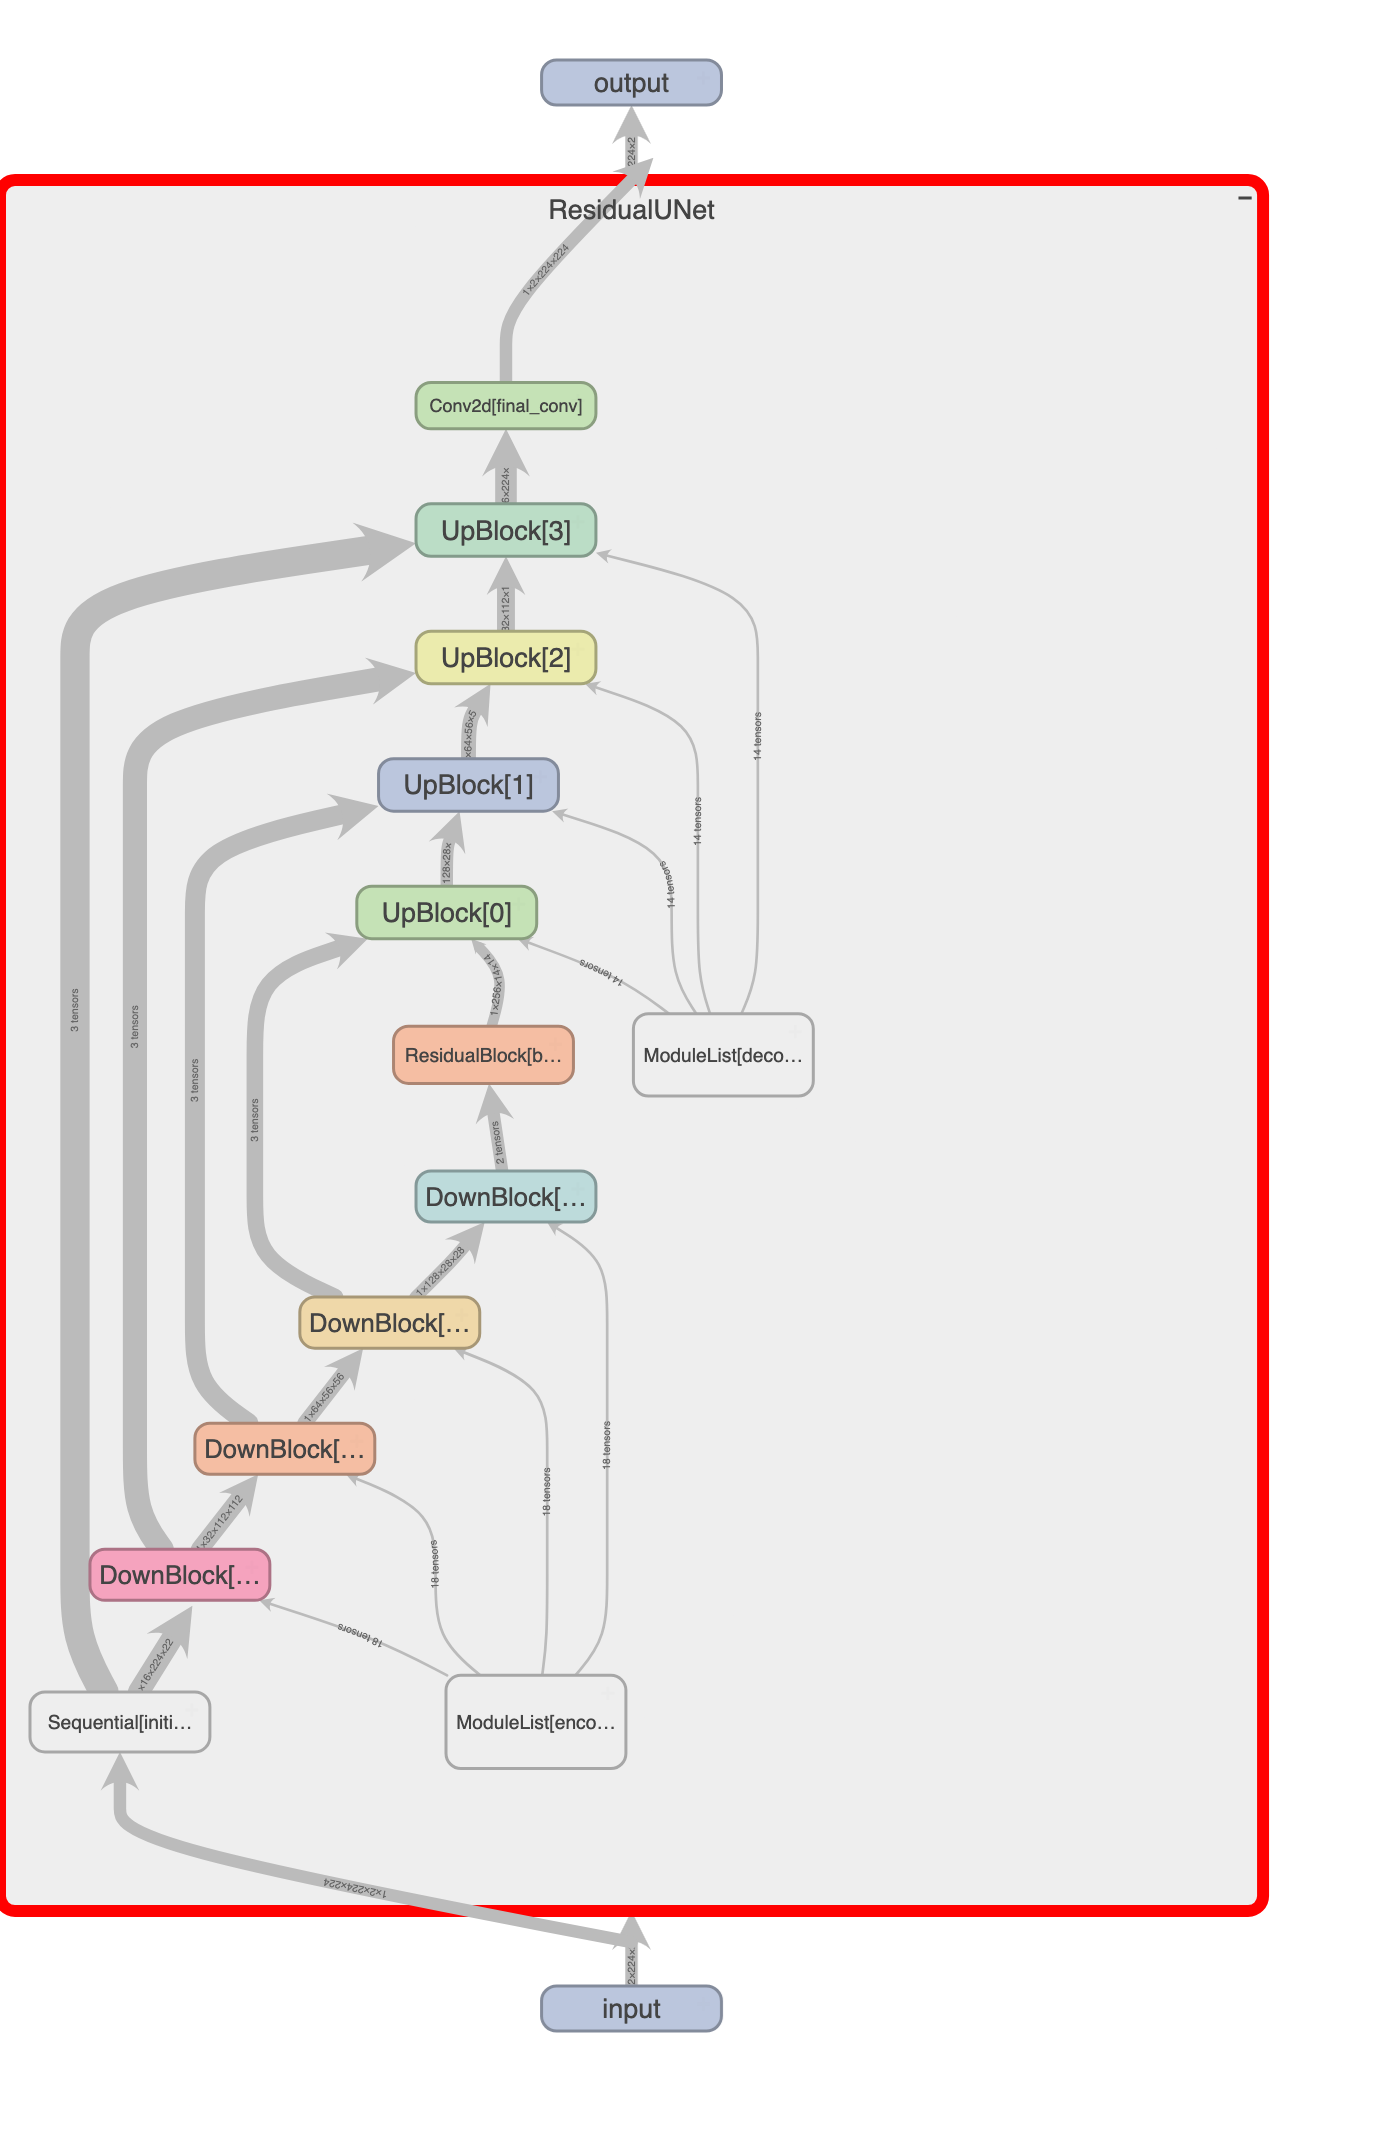
\includegraphics[width=0.45\textwidth]{images/unet_experiment_graph.png}
\end{frame}

\begin{frame}{Model and hyperparameters}
    Even the best model couldn't get decent results with the suggested MSE loss, so we adopted a combined loss approach
    \begin{columns}
        \column{0.5\textwidth}
            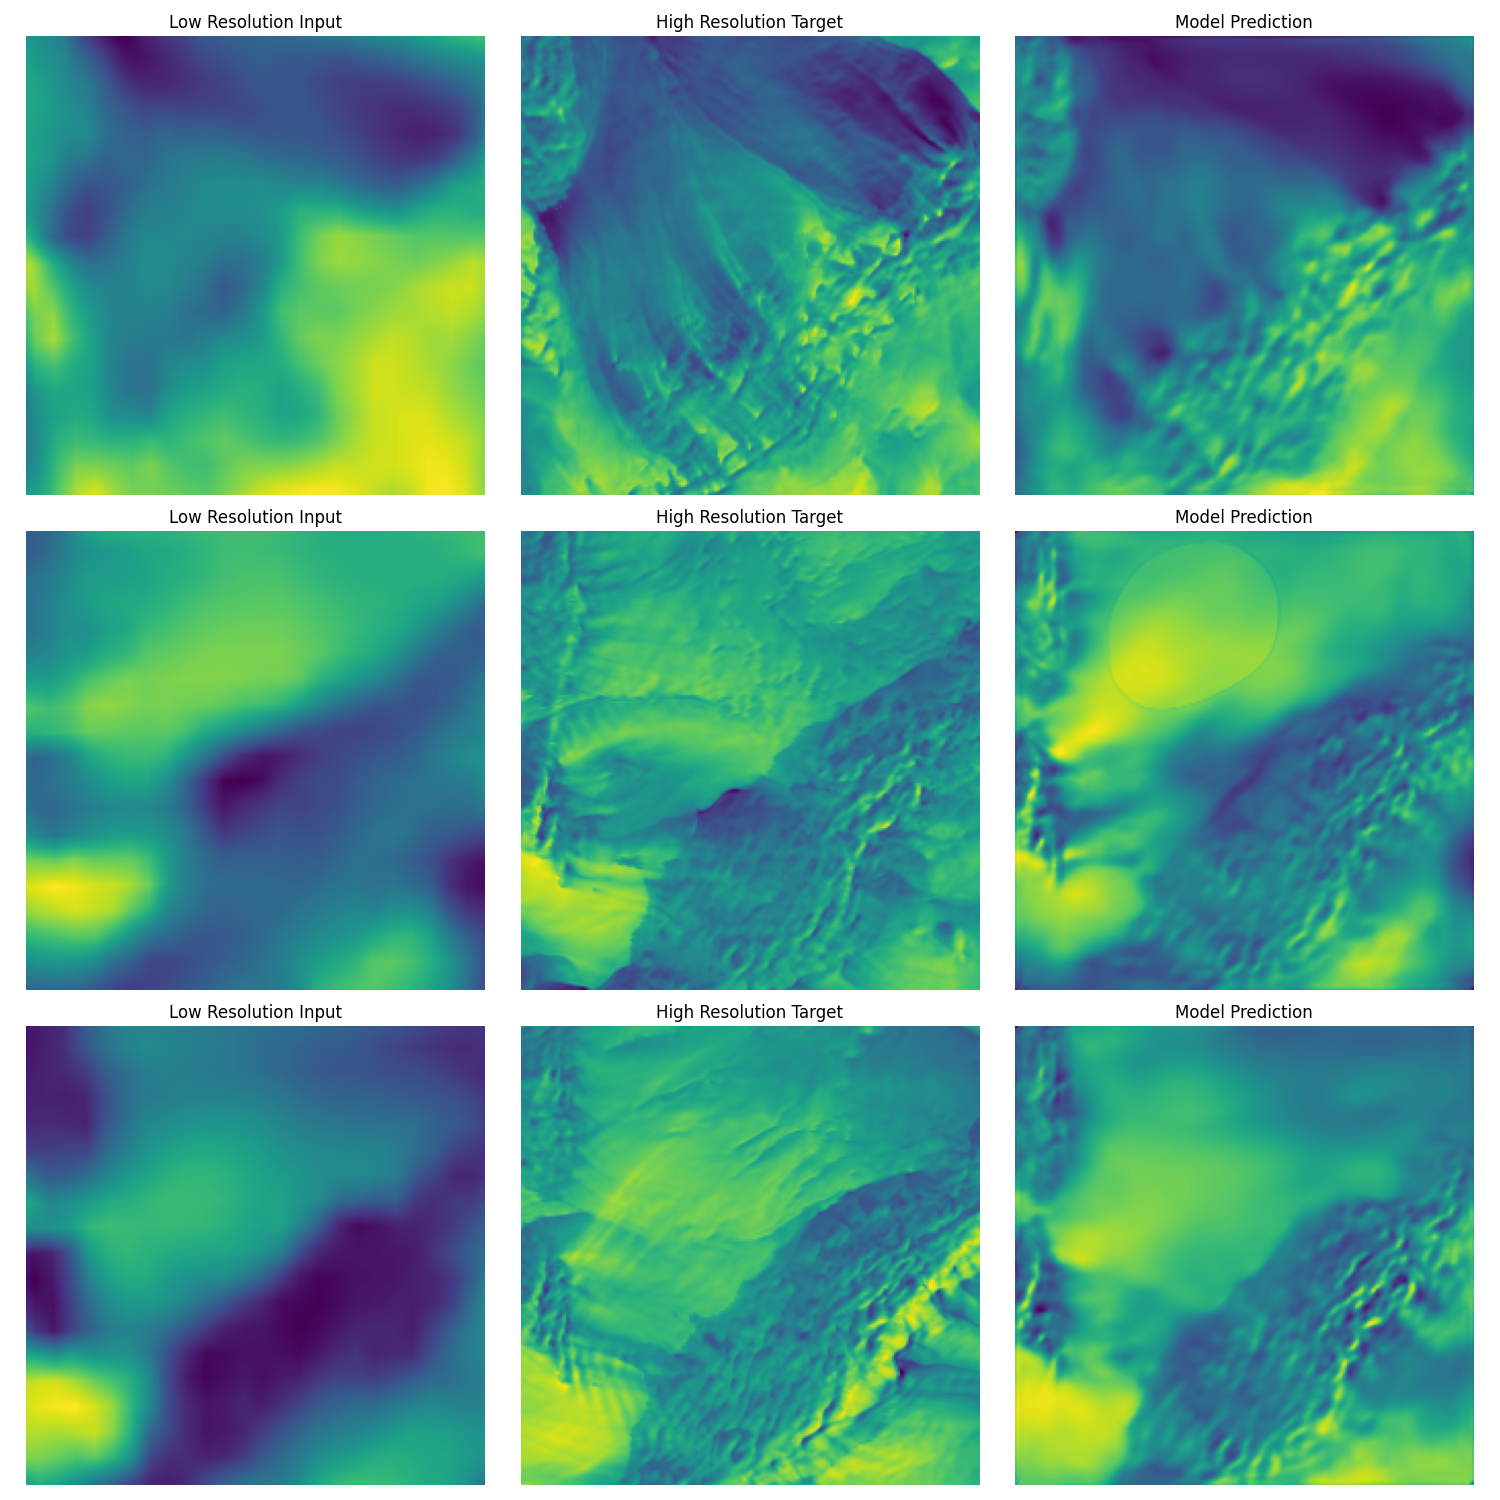
\includegraphics[width=\linewidth]{images/unet_vectors_l1ssim_loss_200_epochs_4_batch_1em3_lr_1em5_weightdecay.png}
            \newline
            \centering \small L1 + SSIM loss. SSIM: \texttt{0.7556}
        \column{0.5\textwidth}
            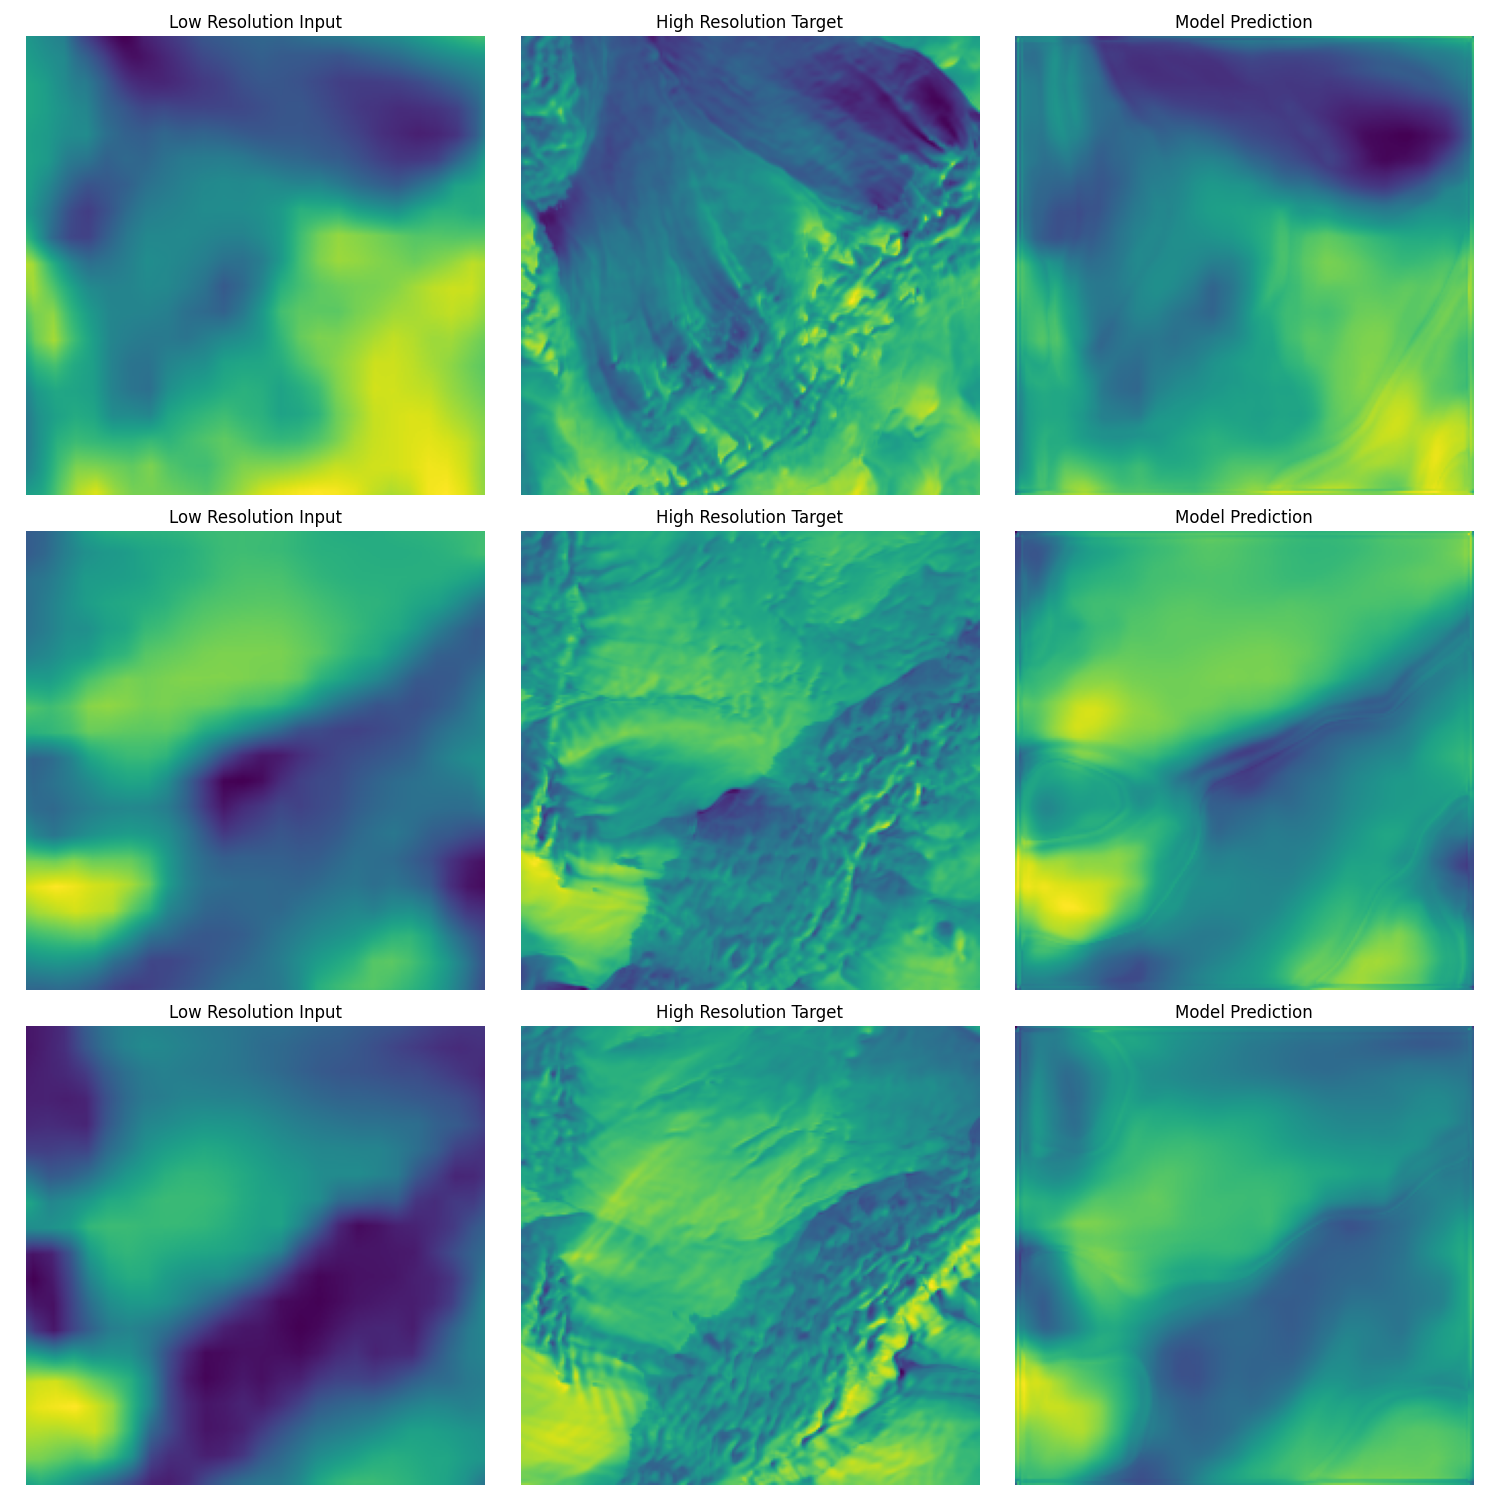
\includegraphics[width=\linewidth]{images/unet_vectors_mse_loss_200_epochs_4_batch_1em3_lr_1em5_weightdecay.png}
            \newline
            \centering \small MSE loss. SSIM: \texttt{0.7022}
    \end{columns}
\end{frame}

\begin{frame}[fragile]{Model and hyperparameters}
    \begin{lstlisting}
    class L1SSIMLoss(nn.Module):
    def __init__(self, alpha=0.85, ssim_window_size=11, ssim_data_range=1.0, ssim_channel=1):
        super(L1SSIMLoss, self).__init__()
        self.alpha = alpha
        self.l1_loss = nn.L1Loss() # Mean Absolute Error
        self.ssim_loss_fn = SSIMLoss(window_size=ssim_window_size, data_range=ssim_data_range, channel=ssim_channel)

    def forward(self, y_pred, y_true):
        ssim_val_loss = self.ssim_loss_fn(y_pred, y_true)
        l1_val_loss = self.l1_loss(y_pred, y_true)
        
        combined_loss = self.alpha * ssim_val_loss + (1 - self.alpha) * l1_val_loss
        return combined_loss
    \end{lstlisting}
\end{frame}

\begin{frame}{Model and hyperparameters}
    % SCELTA DEGLI IPERPARAMETRI CON TABELLA TRAINING
\end{frame}

% MATTEO
\begin{frame}{Training}
% training falliti + poi come ce la siamo cavata
\end{frame}

% FEDE
\begin{frame}{Results}
% mostrare i risultati finali per entrambi + un commento sulla differenza tra training locale con 100 immagini e training su colab con 1000
\end{frame}

% MARZIA
\begin{frame}{Final Considerations}
% come ci aspettavamo la rappresentazione con vettori e' quella migliore e quella con intensita' e direzione fa schifo al cazzo
\end{frame}

\begin{frame}
    \frametitle{References}
    \printbibliography
\end{frame}
\end{document}
